\subsection{Беззнаковые числа}

\begin{frame}
	\tableofcontents[currentsection,currentsubsection]
\end{frame}

\begin{frame}{Один байт}
	\begin{align*}
		239 = 128 + 16 + 4 + 2
	\end{align*}
	Есть младшие знаки, есть старшие.

	Всё в двоичной системе (привет из школы).
	Пока работаем в пределах одного байта.

	Пока все результаты от $0$ до $255$, нет никаких проблем "--- считаем и считаем.
	Что делать, если произошло переполнение (overflow/underflow)?
	Результат точно не сохраним.
	Можно кинуть ошибку, можно откинуть какие-нибудь знаки и это обозначить.
	Если откинем младшие, то $254+1-1\neq 254$, неудобно, куча случаев вылезет.
\end{frame}

\begin{frame}
	\begin{center}
		
\includegraphics[scale=0.3]{will-i-use-algebra.jpg}
	\end{center}
\end{frame}

\begin{frame}
	А вот если считаем, что откидываем старшие, то получаем кольцо $\mathbb{Z}/256\mathbb{Z}$.

	\begin{center}
		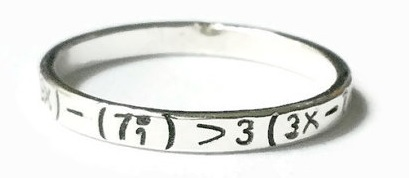
\includegraphics[scale=1]{math-ring.jpg}
	\end{center}

	Сложение, вычитание, умножение прекрасно определены и непротиворечивы.
	Можно делать что угодно, и мы всегда получим корректный результат по модулю 256.
	В железе реализовать просто.
\end{frame}

\begin{frame}{Деление}
	С делением хуже (деление "--- обратное к умножению).
	После взятия по модулю иногда можно однозначно восстановить ответ, а иногда нет (на алгебре расскажут, когда):
	\begin{align*}
	    34 / 17 &= 2 \\
		4386 / 17 &= 258 = 2 \mod 256 \\
		48 / 4 &= 12 \\
		\underbrace{(256+48)}_{304} / 4 &= 76 \\
	\end{align*}
	Поэтому деление всегда считает, что у нас числа помещаются, и делим мы с остатком.
\end{frame}
